\section{Supplied routing: ten 48-qubit workloads}
\begin{center}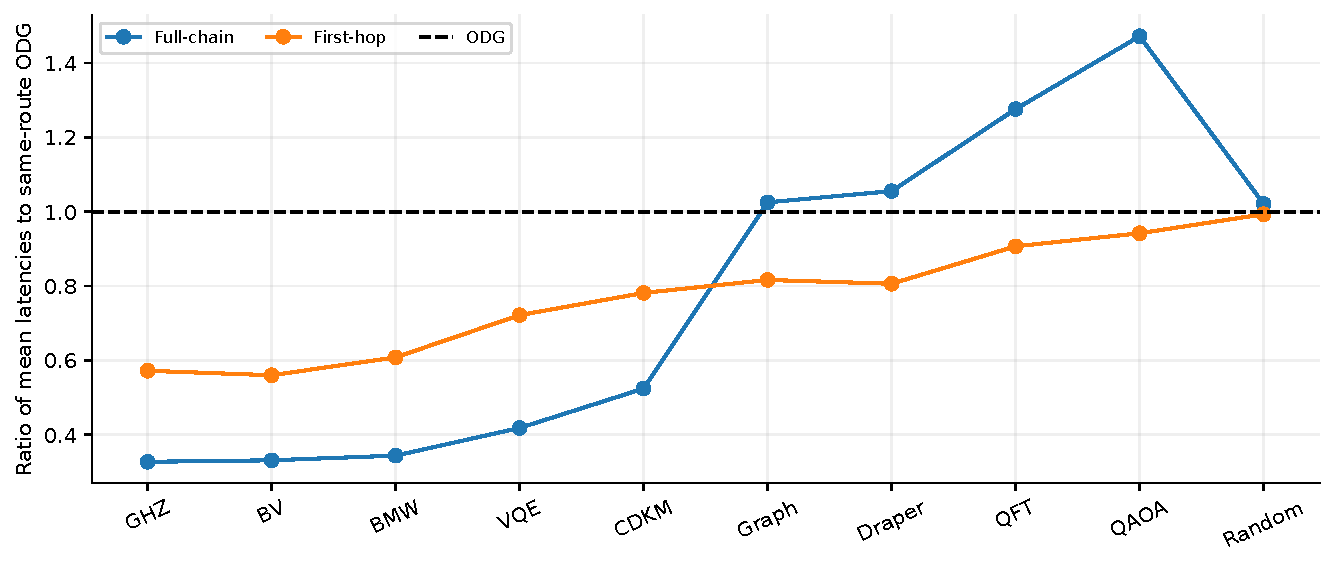
\includegraphics[width=\linewidth,height=0.37\textheight,keepaspectratio]{figures/generalisation_original.pdf}\captionof{figure}{Ratios of seed means, three physics seeds per policy. Workload categories have no continuous order. Ratios have no confidence intervals here.}\end{center}

\begin{center}\small
\begin{longtable}{lrr}
\caption{Exact latency ratios plotted above; values below one favour the listed Dynamic policy.}\\
\toprule
Workload & Full-chain & First-hop \\
\midrule\endfirsthead
\toprule
Workload & Full-chain & First-hop \\
\midrule\endhead
GHZ & 0.3274 & 0.5723 \\
BV & 0.3315 & 0.5602 \\
BMW & 0.3441 & 0.6084 \\
VQE & 0.4184 & 0.7218 \\
CDKM & 0.5244 & 0.7816 \\
Graph & 1.0252 & 0.8165 \\
Draper & 1.0553 & 0.8062 \\
QFT & 1.2759 & 0.9070 \\
QAOA & 1.4718 & 0.9420 \\
Random & 1.0209 & 0.9932 \\
\bottomrule\end{longtable}\end{center}
{\footnotesize \href{https://github.com/sanjeevkrishnaa/Compiler-Driven-ACE/blob/codex/ace-scheduler-correctness/docs/latex/oct25_pre_golden/data/generalisation.csv}{Complete CSV: generalisation}. }

\begin{center}\small
\begin{longtable}{lrrr}
\caption{Latency (ms), mean $\pm$ SD across three seeds.}\\
\toprule
Workload & ODG & Full-chain & First-hop \\
\midrule\endfirsthead
\toprule
Workload & ODG & Full-chain & First-hop \\
\midrule\endhead
GHZ & $1.413 \pm 0.131$ & $0.463 \pm 0.000$ & $0.808 \pm 0.070$ \\
BV & $1.440 \pm 0.142$ & $0.477 \pm 0.058$ & $0.807 \pm 0.054$ \\
BMW & $1.315 \pm 0.055$ & $0.452 \pm 0.004$ & $0.800 \pm 0.016$ \\
VQE & $1.346 \pm 0.046$ & $0.563 \pm 0.023$ & $0.971 \pm 0.051$ \\
CDKM & $1.339 \pm 0.028$ & $0.702 \pm 0.030$ & $1.046 \pm 0.018$ \\
Graph & $1.391 \pm 0.075$ & $1.426 \pm 0.217$ & $1.136 \pm 0.040$ \\
Draper & $1.339 \pm 0.021$ & $1.413 \pm 0.038$ & $1.079 \pm 0.010$ \\
QFT & $1.414 \pm 0.018$ & $1.804 \pm 0.145$ & $1.282 \pm 0.022$ \\
QAOA & $1.362 \pm 0.013$ & $2.005 \pm 0.068$ & $1.283 \pm 0.055$ \\
Random & $1.310 \pm 0.007$ & $1.338 \pm 0.012$ & $1.301 \pm 0.023$ \\
\bottomrule\end{longtable}\end{center}
{\footnotesize \href{https://github.com/sanjeevkrishnaa/Compiler-Driven-ACE/blob/codex/ace-scheduler-correctness/docs/latex/oct25_pre_golden/data/generalisation.csv}{Complete CSV: generalisation}. }

\begin{center}\small
\begin{longtable}{lrrr}
\caption{Makespan (s), mean $\pm$ SD across three seeds.}\\
\toprule
Workload & ODG & Full-chain & First-hop \\
\midrule\endfirsthead
\toprule
Workload & ODG & Full-chain & First-hop \\
\midrule\endhead
GHZ & $0.204 \pm 0.003$ & $0.181 \pm 0.000$ & $0.189 \pm 0.002$ \\
BV & $0.761 \pm 0.004$ & $0.737 \pm 0.001$ & $0.745 \pm 0.001$ \\
BMW & $6.219 \pm 0.008$ & $6.095 \pm 0.001$ & $6.145 \pm 0.002$ \\
VQE & $0.338 \pm 0.006$ & $0.277 \pm 0.001$ & $0.315 \pm 0.004$ \\
CDKM & $3.364 \pm 0.013$ & $3.076 \pm 0.015$ & $3.232 \pm 0.007$ \\
Graph & $0.129 \pm 0.004$ & $0.119 \pm 0.004$ & $0.121 \pm 0.001$ \\
Draper & $2.388 \pm 0.010$ & $2.283 \pm 0.025$ & $2.271 \pm 0.006$ \\
QFT & $2.116 \pm 0.045$ & $2.150 \pm 0.065$ & $2.059 \pm 0.007$ \\
QAOA & $2.082 \pm 0.028$ & $2.347 \pm 0.023$ & $2.003 \pm 0.024$ \\
Random & $14.990 \pm 0.031$ & $14.284 \pm 0.035$ & $14.490 \pm 0.100$ \\
\bottomrule\end{longtable}\end{center}
{\footnotesize \href{https://github.com/sanjeevkrishnaa/Compiler-Driven-ACE/blob/codex/ace-scheduler-correctness/docs/latex/oct25_pre_golden/data/generalisation.csv}{Complete CSV: generalisation}. }

\begin{center}\small
\begin{longtable}{lrrr}
\caption{Delivered fidelity, mean $\pm$ SD across three seeds.}\\
\toprule
Workload & ODG & Full-chain & First-hop \\
\midrule\endfirsthead
\toprule
Workload & ODG & Full-chain & First-hop \\
\midrule\endhead
GHZ & $0.9498 \pm 0.0000$ & $0.9417 \pm 0.0002$ & $0.9451 \pm 0.0002$ \\
BV & $0.9498 \pm 0.0000$ & $0.9416 \pm 0.0002$ & $0.9450 \pm 0.0001$ \\
BMW & $0.9498 \pm 0.0000$ & $0.9415 \pm 0.0001$ & $0.9450 \pm 0.0001$ \\
VQE & $0.9498 \pm 0.0000$ & $0.9422 \pm 0.0001$ & $0.9460 \pm 0.0001$ \\
CDKM & $0.9498 \pm 0.0000$ & $0.9439 \pm 0.0003$ & $0.9474 \pm 0.0000$ \\
Graph & $0.9498 \pm 0.0000$ & $0.9446 \pm 0.0010$ & $0.9485 \pm 0.0002$ \\
Draper & $0.9498 \pm 0.0000$ & $0.9444 \pm 0.0004$ & $0.9469 \pm 0.0001$ \\
QFT & $0.9498 \pm 0.0000$ & $0.9451 \pm 0.0005$ & $0.9481 \pm 0.0000$ \\
QAOA & $0.9498 \pm 0.0000$ & $0.9457 \pm 0.0003$ & $0.9478 \pm 0.0000$ \\
Random & $0.9498 \pm 0.0000$ & $0.9472 \pm 0.0001$ & $0.9483 \pm 0.0000$ \\
\bottomrule\end{longtable}\end{center}
{\footnotesize \href{https://github.com/sanjeevkrishnaa/Compiler-Driven-ACE/blob/codex/ace-scheduler-correctness/docs/latex/oct25_pre_golden/data/generalisation.csv}{Complete CSV: generalisation}. }

\begin{center}\small
\begin{longtable}{lrrr}
\caption{Readiness fraction, mean $\pm$ SD across three seeds.}\\
\toprule
Workload & ODG & Full-chain & First-hop \\
\midrule\endfirsthead
\toprule
Workload & ODG & Full-chain & First-hop \\
\midrule\endhead
GHZ & $0.000 \pm 0.000$ & $1.000 \pm 0.000$ & $0.625 \pm 0.000$ \\
BV & $0.000 \pm 0.000$ & $0.987 \pm 0.023$ & $0.627 \pm 0.023$ \\
BMW & $0.000 \pm 0.000$ & $0.998 \pm 0.004$ & $0.625 \pm 0.000$ \\
VQE & $0.000 \pm 0.000$ & $0.939 \pm 0.015$ & $0.471 \pm 0.000$ \\
CDKM & $0.000 \pm 0.000$ & $0.703 \pm 0.032$ & $0.332 \pm 0.003$ \\
Graph & $0.000 \pm 0.000$ & $0.561 \pm 0.088$ & $0.250 \pm 0.023$ \\
Draper & $0.000 \pm 0.000$ & $0.523 \pm 0.029$ & $0.353 \pm 0.003$ \\
QFT & $0.000 \pm 0.000$ & $0.409 \pm 0.056$ & $0.223 \pm 0.006$ \\
QAOA & $0.000 \pm 0.000$ & $0.350 \pm 0.018$ & $0.252 \pm 0.003$ \\
Random & $0.000 \pm 0.000$ & $0.285 \pm 0.007$ & $0.216 \pm 0.003$ \\
\bottomrule\end{longtable}\end{center}
{\footnotesize \href{https://github.com/sanjeevkrishnaa/Compiler-Driven-ACE/blob/codex/ace-scheduler-correctness/docs/latex/oct25_pre_golden/data/generalisation.csv}{Complete CSV: generalisation}. }

\begin{center}\small
\begin{longtable}{lrrr}
\caption{Compiler waste (percent), mean $\pm$ SD across three seeds.}\\
\toprule
Workload & ODG & Full-chain & First-hop \\
\midrule\endfirsthead
\toprule
Workload & ODG & Full-chain & First-hop \\
\midrule\endhead
GHZ & n/a & $0.000 \pm 0.000$ & $0.000 \pm 0.000$ \\
BV & n/a & $0.000 \pm 0.000$ & $0.000 \pm 0.000$ \\
BMW & n/a & $0.231 \pm 0.401$ & $0.000 \pm 0.000$ \\
VQE & n/a & $0.340 \pm 0.589$ & $0.000 \pm 0.000$ \\
CDKM & n/a & $2.086 \pm 0.837$ & $1.062 \pm 0.368$ \\
Graph & n/a & $4.527 \pm 2.777$ & $6.349 \pm 7.274$ \\
Draper & n/a & $1.157 \pm 0.491$ & $0.216 \pm 0.216$ \\
QFT & n/a & $1.335 \pm 0.446$ & $1.593 \pm 0.563$ \\
QAOA & n/a & $1.239 \pm 0.215$ & $0.509 \pm 0.129$ \\
Random & n/a & $4.187 \pm 0.142$ & $4.819 \pm 0.211$ \\
\bottomrule\end{longtable}\end{center}
{\footnotesize \href{https://github.com/sanjeevkrishnaa/Compiler-Driven-ACE/blob/codex/ace-scheduler-correctness/docs/latex/oct25_pre_golden/data/generalisation.csv}{Complete CSV: generalisation}. }

\section{XY routing: ten 48-qubit workloads}
\begin{center}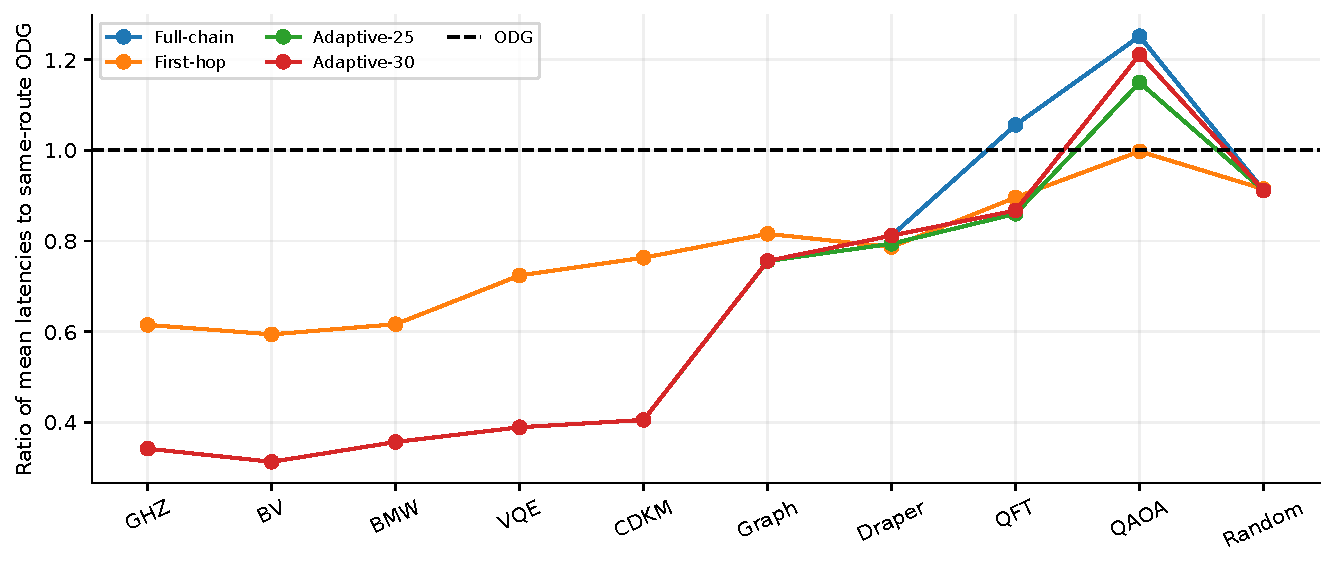
\includegraphics[width=\linewidth,height=0.37\textheight,keepaspectratio]{figures/generalisation_xy.pdf}\captionof{figure}{Ratios of seed means, three physics seeds per policy. Workload categories have no continuous order. Ratios have no confidence intervals here.}\end{center}

\begin{center}\small
\begin{longtable}{lrrrr}
\caption{Exact latency ratios plotted above; values below one favour the listed Dynamic policy.}\\
\toprule
Workload & Full-chain & First-hop & Adaptive-25 & Adaptive-30 \\
\midrule\endfirsthead
\toprule
Workload & Full-chain & First-hop & Adaptive-25 & Adaptive-30 \\
\midrule\endhead
GHZ & 0.3419 & 0.6150 & 0.3419 & 0.3419 \\
BV & 0.3130 & 0.5940 & 0.3130 & 0.3130 \\
BMW & 0.3567 & 0.6165 & 0.3567 & 0.3567 \\
VQE & 0.3891 & 0.7239 & 0.3891 & 0.3891 \\
CDKM & 0.4053 & 0.7630 & 0.4053 & 0.4053 \\
Graph & 0.7560 & 0.8158 & 0.7557 & 0.7560 \\
Draper & 0.8119 & 0.7867 & 0.7939 & 0.8119 \\
QFT & 1.0561 & 0.8961 & 0.8601 & 0.8674 \\
QAOA & 1.2516 & 0.9977 & 1.1495 & 1.2111 \\
Random & 0.9116 & 0.9146 & 0.9115 & 0.9116 \\
\bottomrule\end{longtable}\end{center}
{\footnotesize \href{https://github.com/sanjeevkrishnaa/Compiler-Driven-ACE/blob/codex/ace-scheduler-correctness/docs/latex/oct25_pre_golden/data/generalisation.csv}{Complete CSV: generalisation}. }

\begin{center}\small
\begin{longtable}{lrrrrr}
\caption{Latency (ms), mean $\pm$ SD across three seeds.}\\
\toprule
Workload & ODG & Full-chain & First-hop & Adaptive-25 & Adaptive-30 \\
\midrule\endfirsthead
\toprule
Workload & ODG & Full-chain & First-hop & Adaptive-25 & Adaptive-30 \\
\midrule\endhead
GHZ & $1.353 \pm 0.148$ & $0.463 \pm 0.000$ & $0.832 \pm 0.106$ & $0.463 \pm 0.000$ & $0.463 \pm 0.000$ \\
BV & $1.419 \pm 0.140$ & $0.444 \pm 0.000$ & $0.843 \pm 0.083$ & $0.444 \pm 0.000$ & $0.444 \pm 0.000$ \\
BMW & $1.268 \pm 0.039$ & $0.452 \pm 0.004$ & $0.782 \pm 0.017$ & $0.452 \pm 0.004$ & $0.452 \pm 0.004$ \\
VQE & $1.298 \pm 0.039$ & $0.505 \pm 0.021$ & $0.940 \pm 0.033$ & $0.505 \pm 0.021$ & $0.505 \pm 0.021$ \\
CDKM & $1.349 \pm 0.025$ & $0.547 \pm 0.009$ & $1.030 \pm 0.032$ & $0.547 \pm 0.009$ & $0.547 \pm 0.009$ \\
Graph & $1.431 \pm 0.093$ & $1.082 \pm 0.090$ & $1.168 \pm 0.043$ & $1.082 \pm 0.177$ & $1.082 \pm 0.090$ \\
Draper & $1.342 \pm 0.013$ & $1.090 \pm 0.033$ & $1.056 \pm 0.021$ & $1.066 \pm 0.062$ & $1.090 \pm 0.033$ \\
QFT & $1.383 \pm 0.016$ & $1.461 \pm 0.198$ & $1.240 \pm 0.050$ & $1.190 \pm 0.034$ & $1.200 \pm 0.055$ \\
QAOA & $1.345 \pm 0.014$ & $1.683 \pm 0.040$ & $1.342 \pm 0.091$ & $1.546 \pm 0.128$ & $1.629 \pm 0.110$ \\
Random & $1.312 \pm 0.005$ & $1.196 \pm 0.005$ & $1.200 \pm 0.003$ & $1.196 \pm 0.009$ & $1.196 \pm 0.005$ \\
\bottomrule\end{longtable}\end{center}
{\footnotesize \href{https://github.com/sanjeevkrishnaa/Compiler-Driven-ACE/blob/codex/ace-scheduler-correctness/docs/latex/oct25_pre_golden/data/generalisation.csv}{Complete CSV: generalisation}. }

\begin{center}\small
\begin{longtable}{lrrrrr}
\caption{Makespan (s), mean $\pm$ SD across three seeds.}\\
\toprule
Workload & ODG & Full-chain & First-hop & Adaptive-25 & Adaptive-30 \\
\midrule\endfirsthead
\toprule
Workload & ODG & Full-chain & First-hop & Adaptive-25 & Adaptive-30 \\
\midrule\endhead
GHZ & $0.202 \pm 0.004$ & $0.181 \pm 0.000$ & $0.190 \pm 0.003$ & $0.181 \pm 0.000$ & $0.181 \pm 0.000$ \\
BV & $0.760 \pm 0.003$ & $0.736 \pm 0.000$ & $0.746 \pm 0.002$ & $0.736 \pm 0.000$ & $0.736 \pm 0.000$ \\
BMW & $6.213 \pm 0.006$ & $6.095 \pm 0.001$ & $6.143 \pm 0.002$ & $6.095 \pm 0.001$ & $6.095 \pm 0.001$ \\
VQE & $0.337 \pm 0.006$ & $0.273 \pm 0.001$ & $0.314 \pm 0.004$ & $0.273 \pm 0.001$ & $0.273 \pm 0.001$ \\
CDKM & $3.371 \pm 0.013$ & $3.008 \pm 0.003$ & $3.227 \pm 0.015$ & $3.008 \pm 0.003$ & $3.008 \pm 0.003$ \\
Graph & $0.128 \pm 0.003$ & $0.113 \pm 0.003$ & $0.122 \pm 0.004$ & $0.114 \pm 0.005$ & $0.113 \pm 0.003$ \\
Draper & $2.389 \pm 0.015$ & $2.176 \pm 0.009$ & $2.262 \pm 0.023$ & $2.163 \pm 0.032$ & $2.176 \pm 0.009$ \\
QFT & $2.101 \pm 0.028$ & $2.005 \pm 0.060$ & $2.050 \pm 0.037$ & $1.980 \pm 0.035$ & $1.955 \pm 0.033$ \\
QAOA & $2.056 \pm 0.026$ & $2.139 \pm 0.009$ & $2.045 \pm 0.050$ & $2.082 \pm 0.062$ & $2.109 \pm 0.057$ \\
Random & $15.043 \pm 0.082$ & $13.514 \pm 0.072$ & $14.085 \pm 0.007$ & $13.535 \pm 0.043$ & $13.514 \pm 0.072$ \\
\bottomrule\end{longtable}\end{center}
{\footnotesize \href{https://github.com/sanjeevkrishnaa/Compiler-Driven-ACE/blob/codex/ace-scheduler-correctness/docs/latex/oct25_pre_golden/data/generalisation.csv}{Complete CSV: generalisation}. }

\begin{center}\small
\begin{longtable}{lrrrrr}
\caption{Delivered fidelity, mean $\pm$ SD across three seeds.}\\
\toprule
Workload & ODG & Full-chain & First-hop & Adaptive-25 & Adaptive-30 \\
\midrule\endfirsthead
\toprule
Workload & ODG & Full-chain & First-hop & Adaptive-25 & Adaptive-30 \\
\midrule\endhead
GHZ & $0.9498 \pm 0.0000$ & $0.9416 \pm 0.0003$ & $0.9450 \pm 0.0001$ & $0.9416 \pm 0.0003$ & $0.9416 \pm 0.0003$ \\
BV & $0.9498 \pm 0.0000$ & $0.9418 \pm 0.0003$ & $0.9449 \pm 0.0001$ & $0.9418 \pm 0.0003$ & $0.9418 \pm 0.0003$ \\
BMW & $0.9498 \pm 0.0000$ & $0.9414 \pm 0.0001$ & $0.9449 \pm 0.0001$ & $0.9414 \pm 0.0001$ & $0.9414 \pm 0.0001$ \\
VQE & $0.9498 \pm 0.0000$ & $0.9417 \pm 0.0002$ & $0.9460 \pm 0.0001$ & $0.9417 \pm 0.0002$ & $0.9417 \pm 0.0002$ \\
CDKM & $0.9498 \pm 0.0000$ & $0.9430 \pm 0.0001$ & $0.9475 \pm 0.0001$ & $0.9430 \pm 0.0001$ & $0.9430 \pm 0.0001$ \\
Graph & $0.9498 \pm 0.0000$ & $0.9451 \pm 0.0007$ & $0.9486 \pm 0.0001$ & $0.9458 \pm 0.0008$ & $0.9451 \pm 0.0007$ \\
Draper & $0.9498 \pm 0.0000$ & $0.9443 \pm 0.0004$ & $0.9469 \pm 0.0001$ & $0.9441 \pm 0.0005$ & $0.9443 \pm 0.0004$ \\
QFT & $0.9498 \pm 0.0000$ & $0.9443 \pm 0.0001$ & $0.9480 \pm 0.0000$ & $0.9473 \pm 0.0000$ & $0.9466 \pm 0.0000$ \\
QAOA & $0.9498 \pm 0.0000$ & $0.9459 \pm 0.0004$ & $0.9479 \pm 0.0001$ & $0.9467 \pm 0.0004$ & $0.9463 \pm 0.0003$ \\
Random & $0.9498 \pm 0.0000$ & $0.9468 \pm 0.0000$ & $0.9482 \pm 0.0001$ & $0.9469 \pm 0.0001$ & $0.9468 \pm 0.0000$ \\
\bottomrule\end{longtable}\end{center}
{\footnotesize \href{https://github.com/sanjeevkrishnaa/Compiler-Driven-ACE/blob/codex/ace-scheduler-correctness/docs/latex/oct25_pre_golden/data/generalisation.csv}{Complete CSV: generalisation}. }

\begin{center}\small
\begin{longtable}{lrrrrr}
\caption{Readiness fraction, mean $\pm$ SD across three seeds.}\\
\toprule
Workload & ODG & Full-chain & First-hop & Adaptive-25 & Adaptive-30 \\
\midrule\endfirsthead
\toprule
Workload & ODG & Full-chain & First-hop & Adaptive-25 & Adaptive-30 \\
\midrule\endhead
GHZ & $0.000 \pm 0.000$ & $1.000 \pm 0.000$ & $0.625 \pm 0.000$ & $1.000 \pm 0.000$ & $1.000 \pm 0.000$ \\
BV & $0.000 \pm 0.000$ & $1.000 \pm 0.000$ & $0.640 \pm 0.000$ & $1.000 \pm 0.000$ & $1.000 \pm 0.000$ \\
BMW & $0.000 \pm 0.000$ & $0.998 \pm 0.004$ & $0.625 \pm 0.000$ & $0.998 \pm 0.004$ & $0.998 \pm 0.004$ \\
VQE & $0.000 \pm 0.000$ & $0.974 \pm 0.006$ & $0.471 \pm 0.000$ & $0.974 \pm 0.006$ & $0.974 \pm 0.006$ \\
CDKM & $0.000 \pm 0.000$ & $0.868 \pm 0.021$ & $0.330 \pm 0.008$ & $0.868 \pm 0.021$ & $0.868 \pm 0.021$ \\
Graph & $0.000 \pm 0.000$ & $0.645 \pm 0.023$ & $0.224 \pm 0.026$ & $0.522 \pm 0.040$ & $0.645 \pm 0.023$ \\
Draper & $0.000 \pm 0.000$ & $0.597 \pm 0.047$ & $0.367 \pm 0.002$ & $0.619 \pm 0.053$ & $0.597 \pm 0.047$ \\
QFT & $0.000 \pm 0.000$ & $0.518 \pm 0.036$ & $0.238 \pm 0.002$ & $0.310 \pm 0.005$ & $0.371 \pm 0.007$ \\
QAOA & $0.000 \pm 0.000$ & $0.369 \pm 0.030$ & $0.235 \pm 0.008$ & $0.318 \pm 0.035$ & $0.347 \pm 0.030$ \\
Random & $0.000 \pm 0.000$ & $0.341 \pm 0.003$ & $0.232 \pm 0.009$ & $0.336 \pm 0.009$ & $0.341 \pm 0.003$ \\
\bottomrule\end{longtable}\end{center}
{\footnotesize \href{https://github.com/sanjeevkrishnaa/Compiler-Driven-ACE/blob/codex/ace-scheduler-correctness/docs/latex/oct25_pre_golden/data/generalisation.csv}{Complete CSV: generalisation}. }

\begin{center}\small
\begin{longtable}{lrrrrr}
\caption{Compiler waste (percent), mean $\pm$ SD across three seeds.}\\
\toprule
Workload & ODG & Full-chain & First-hop & Adaptive-25 & Adaptive-30 \\
\midrule\endfirsthead
\toprule
Workload & ODG & Full-chain & First-hop & Adaptive-25 & Adaptive-30 \\
\midrule\endhead
GHZ & n/a & $0.000 \pm 0.000$ & $0.000 \pm 0.000$ & $0.000 \pm 0.000$ & $0.000 \pm 0.000$ \\
BV & n/a & $0.000 \pm 0.000$ & $0.000 \pm 0.000$ & $0.000 \pm 0.000$ & $0.000 \pm 0.000$ \\
BMW & n/a & $0.231 \pm 0.401$ & $0.000 \pm 0.000$ & $0.231 \pm 0.401$ & $0.231 \pm 0.401$ \\
VQE & n/a & $0.971 \pm 0.971$ & $0.000 \pm 0.000$ & $0.971 \pm 0.971$ & $0.971 \pm 0.971$ \\
CDKM & n/a & $1.305 \pm 0.814$ & $2.123 \pm 1.603$ & $1.305 \pm 0.814$ & $1.305 \pm 0.814$ \\
Graph & n/a & $4.774 \pm 2.776$ & $5.000 \pm 5.000$ & $4.317 \pm 4.348$ & $4.774 \pm 2.776$ \\
Draper & n/a & $1.147 \pm 0.519$ & $0.276 \pm 0.120$ & $0.942 \pm 0.455$ & $1.147 \pm 0.519$ \\
QFT & n/a & $0.902 \pm 0.173$ & $1.450 \pm 0.176$ & $1.450 \pm 0.203$ & $1.114 \pm 0.235$ \\
QAOA & n/a & $1.930 \pm 0.662$ & $1.171 \pm 0.152$ & $1.539 \pm 0.529$ & $1.791 \pm 0.481$ \\
Random & n/a & $3.876 \pm 0.021$ & $4.336 \pm 0.536$ & $3.955 \pm 0.152$ & $3.876 \pm 0.021$ \\
\bottomrule\end{longtable}\end{center}
{\footnotesize \href{https://github.com/sanjeevkrishnaa/Compiler-Driven-ACE/blob/codex/ace-scheduler-correctness/docs/latex/oct25_pre_golden/data/generalisation.csv}{Complete CSV: generalisation}. }
